\documentclass[a4paper,10pt,oneside]{article}
\usepackage[polutonikogreek,italian]{babel}
\usepackage[utf8x]{inputenc}
\usepackage{amsmath}
\usepackage{amsthm}
\usepackage{amssymb}
\usepackage{amscd}
\usepackage{graphicx}
\usepackage{float}
\usepackage{array}
\usepackage{rotating}
\usepackage[small]{caption}
\usepackage{lscape}
\usepackage{fancybox}
\usepackage{booktabs}
\parindent0ex 
\renewcommand{\fboxsep}{0.5cm}
\usepackage{hyperref}
\renewcommand{\textfraction}{0.05}
\renewcommand{\topfraction}{0.95}
\renewcommand{\bottomfraction}{0.95}
\renewcommand{\floatpagefraction}{0.35}
\setcounter{totalnumber}{5}
\restylefloat{figure}
\newlength{\drop}

\begin{document}
{\huge Grandezze fisiche e misure sperimentali}
\begin{abstract}
La fisica (dal greco \textgreek{φύσις} natura) è una scienza naturale il cui scopo è l'analisi della natura e quindi dell'universo che ci circonda, in ognuno dei suoi aspetti. Lo strumento da essa utilizzato per la conoscenza del mondo è il metodo sperimentale e le grandezze di cui essa si occupa vengono manipolate in maniera quantitativa tramite la matematica.
\end{abstract}

\vspace{0.5cm}

Ogni teoria fisica nasce dall'osservazione di fenomeni naturali e il suo scopo è di permetterci di predire e comprendere il comportamento del mondo che ci circonda. 
I mezzi matematici di indagine saranno fondamentali per evincere dai dati delle relazioni utili, soltanto tramite un linguaggio quantitativo e formale sarà possibile costruire una teoria coerente, in grado di spiegare i fenomeni osservati in laboratorio: 

\emph{[\ldots] forse stima che la filosofia sia un libro e una fantasia d'un uomo, come l'Iliade e l'Orlando furioso, libri ne' quali la meno importante cosa è che quello che vi è scritto sia vero. Signor Sarsi, la cosa non istà così. La filosofia è scritta in questo grandissimo libro che continuamente ci sta aperto innanzi agli occhi (io dico l’universo), ma non si può intendere se prima non s'impara a intender la lingua, e conoscer i caratteri, ne' quali è scritto. Egli è scritto in lingua matematica, e i caratteri son triangoli, cerchi, ed altre figure geometriche, senza i quali mezi è impossibile a intenderne umanamente parola; senza questi è un aggirarsi vanamente per un oscuro laberinto.}\footnote{Galileo Galilei - Il Saggiatore}

\vspace{0.5cm}

Durante questa prima esperienza  cercheremo, tramite un semplice esperimento, di ricavare una relazione tra il tempo e lo spazio percorso da una pallina in caduta libera.

Allestiremo il laboratorio come in figura [\ref{fig:setup_sperimentale}]:
\begin{figure}[H]
 \centering
 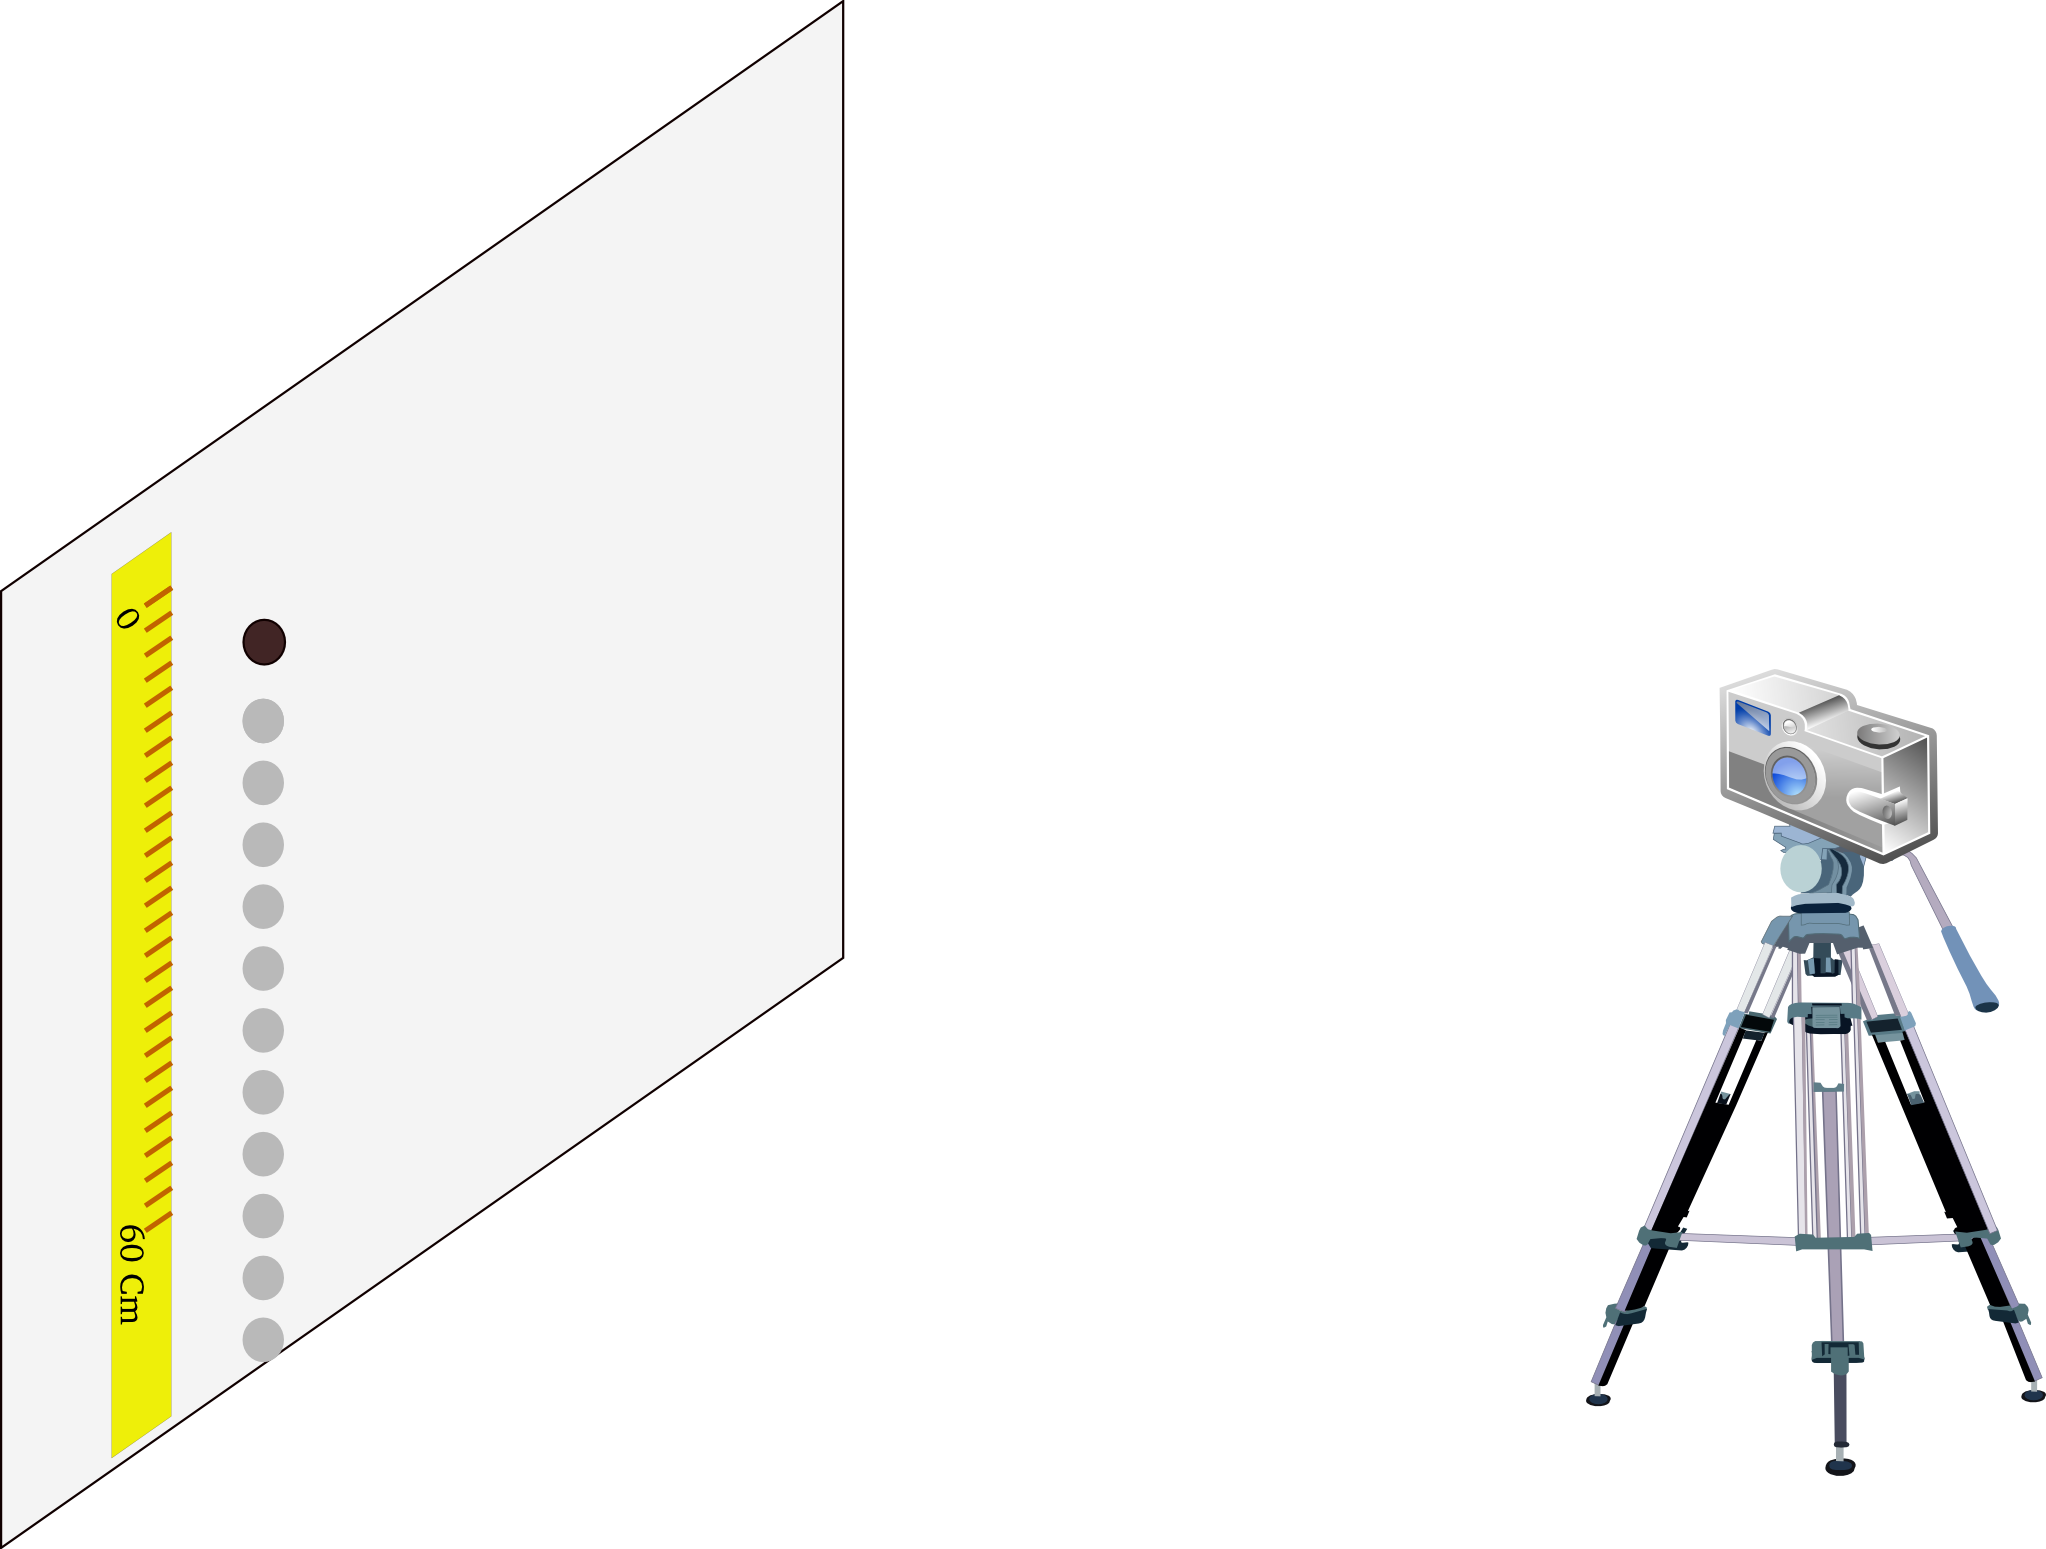
\includegraphics[width=\textwidth]{../immagini/misure_1.png}
 % misure_1.png: 2046x1549 pixel, 201dpi, 25.87x19.59 cm, bb=
 \caption{Una macchina fotografica in grado di girare filmati ad alta frequenza registra la caduta libera di un oggetto}
 \label{fig:setup_sperimentale}
\end{figure}

Per poter effetture una misura indiretta delle posizioni ad un certo istante di tempo, sarà necessario installare un regolo graduato (ad esempio una stecca) alla stessa distanza dalla macchina fotografica della pallina (e quanto più vicino possibile alla traiettora della stessa). Preparato così il laboratorio possiamo registrare la caduta libera della pallina. Prima di iniziare l'analisi dei dati raccolti dobbiamo cercare di misurare accuratamente anche tutte le lunghezze che compaiono nel nostro semplice esperimento:
\begin{itemize}
 \item La lunghezza del regolo
 \item La distanza della macchina fotografica dalla pallina
 \item La quota rispetto al suolo del punto di sgancio
\end{itemize}

\section{Analisi dei dati}

Per l'analisi delle riprese utilizzeremo alcuni software Open Source:
\begin{description}
 \item [ffmpeg] software per la modifica di file video, verrà utilizzato per dividere i filmati in immagini, potete scaricare un installer per Windows a questo indirizzo:
\url{http://www.arachneweb.co.uk/software/windows/avchdview/ffmpeg.html}
\item [Imagemagick] software per la gestione di immagini da linea di comando, verrà utilizzato per combinare le immagini ottenute dalla scomposizione del filmato, potete scaricarlo all'indirizzo: \url{http://www.imagemagick.org/script/binary-releases.php#windows}
\item[Perl] Linguaggio di scripting \url{http://strawberryperl.com}
\item [Gimp] Programma per il foto ritocco \url{http://gimp-win.sourceforge.net/stable.html}
\end{description}


\section{Estrazione delle immagini dal filmato}

Creiamo una directory ad es \verb#c:\laboratorio\video_1# in cui copieremo il video scelto, apriamo quindi un prompt dei comandi tramite il menu esegui digitando \verb#cmd# nella casella di testo associata. Per gli spostamenti da una directory all'altra useremo il comando \verb#cd#:
\begin{verbatim}
cd c:\laboratorio\video_1
\end{verbatim}

ora ci troviamo all'interno della directory creata precedentemente e possiamo utilizzare \verb#ffmpeg# per suddividere il filmato in singoli fotogrammi.
Nell'esempio che potete scaricare da \url{http://cartan.e-moka.net} abbiamo utilizzato il filmato \verb#test_pallina.avi#:
\begin{verbatim}
 ffmpeg -i test_pallina.avi fotogramma%d.png
\end{verbatim}
quando ffmpeg avrà terminato di dividere il filmato, nella directory di lavoro saranno presenti tanti file png quanti sono i fotogrammi del file AVI di partenza. Il file in esame è stato suddiviso in un certo numero di immagini png, guardandole possiamo notare come le prime della serie e le ultime non presentino alcun moto della pallina, tutte queste immagini dovranno essere cancellate.
Ora copiamo il file \verb#out.png# che potete trovare in rete\footnote{È chiaramente possibile creare questo file con qualsiasi editor di immagini, si tratta semplicemente di un'immagine bianca} all'interno della directory ed eseguiamo lo script Perl \verb#combine.pl# che avrete scaricato assieme al file out.png (e copiato all'interno della directory in cui si trova il file Avi):
\begin{verbatim}
#!/usr/bin/perl
use strict;
opendir DIR,".";
while (my $filename=readdir(DIR)){
  if ($filename=~m/png/){
    print $filename,"\n";
    system("convert  out.png $filename  -compose Darken -composite out.png");
	}
}
\end{verbatim}
lo script in Perl può essere eseguito semplicemente tramite un doppio click sulla sua icona.
In poco tempo Imagemagick assemblerà le immagini\footnote{Le immagini sono assemblate tramite un processo di \textsl{darkening}} permettendoci di vedere la traiettoria sovraimposta all'immagine del laboratorio.

\section{Misura delle posizioni in pixel della pallina ad un certo istante di tempo}

L'immagine ottenuta precedentemente dovrà ora essere analizzata. Utilizzeremo lo strumento puntatore di Gimp per ottenere la posizione dei centri delle immagini della pallina. In questo primo esempio ci interesseremo unicamente alla coordinata verticale. L'intervallo temporale tra due immagini verrà ricavato dalla frequenza del video. Se ad esempio abbiamo utilizzato un filmato a  $240Hz$ e mantenuto un'immagine su due, l'intervallo temporale sarà $\Delta t=2*\frac{1}{240}s$

\begin{table}[H]
\begin{center}
\begin{tabular}{ll}\toprule
$t$& $y_{im}$\\ \midrule
0s& 210\\
0.008s&218\\
0.017s&226\\
\ldots&\ldots \\ \bottomrule
\end{tabular}\caption{Posizioni in pixel dei primi tre centri della pallina}\label{tab:postab1}
\end{center}
\end{table}
Siccome il punto di sgancio della pallina non coincide con lo zero della coordinata $y$ nel sistema di riferimento dell'immagine dobbiamo applicare la [\ref{tras}] ad ogni valore $y_{im}$ misurato:
\begin{equation}\label{tras}
 y^*_{im}=y_{im}-y_b
\end{equation}
dove $y_b$ è la coordinata $y$,  nel sistema di riferimento dell'immagine, del punto di sgancio.

Per trasformare le coordinate in pixel in coordinate in cm dobbiamo determinare la risoluzione dell'immagine, cosa che possiamo fare misurando la lunghezza in pixel della stecca,  posizionata in corrispondenza della traiettoria della pallina. 
Se la stecca utilizzata misura $60cm$  e la sua lunghezza sull'immagine è di 130 pixel la risoluzione risulterà:
\begin{equation}
 \delta=\frac{60}{130}\ cm\cdot pixel^{-1}\sim 0.46\ cm\cdot pixel ^{-1}
\end{equation}


 Utilizzando l'informazione relativa alla risoluzione dell'immagine possiamo aggiungere una colonna alla tabella [\ref{tab:postab1}]: lo spostamento $y$ reale rispetto al punto di sgancio della pallina.
\begin{table}[H]
\begin{center}
\begin{tabular}{lll}\toprule
$t$& $y_{im}$ & $s_y$\\ \midrule
0s& 210&0 cm\\
0.008s&218&4.3 cm\\
0.017s&226&8 cm\\
\ldots&\ldots&\ldots\\ \bottomrule
\end{tabular}\caption{Posizioni in cm dei primi tre centri della pallina}\label{tab:postab1}
\end{center}
\end{table}
Se riportiamo in un grafico i dati otteniamo una spezzata il cui andamento sarà simile a quello in figura [\ref{fig:grafico_dati}]
\begin{figure}[H]
 \centering
 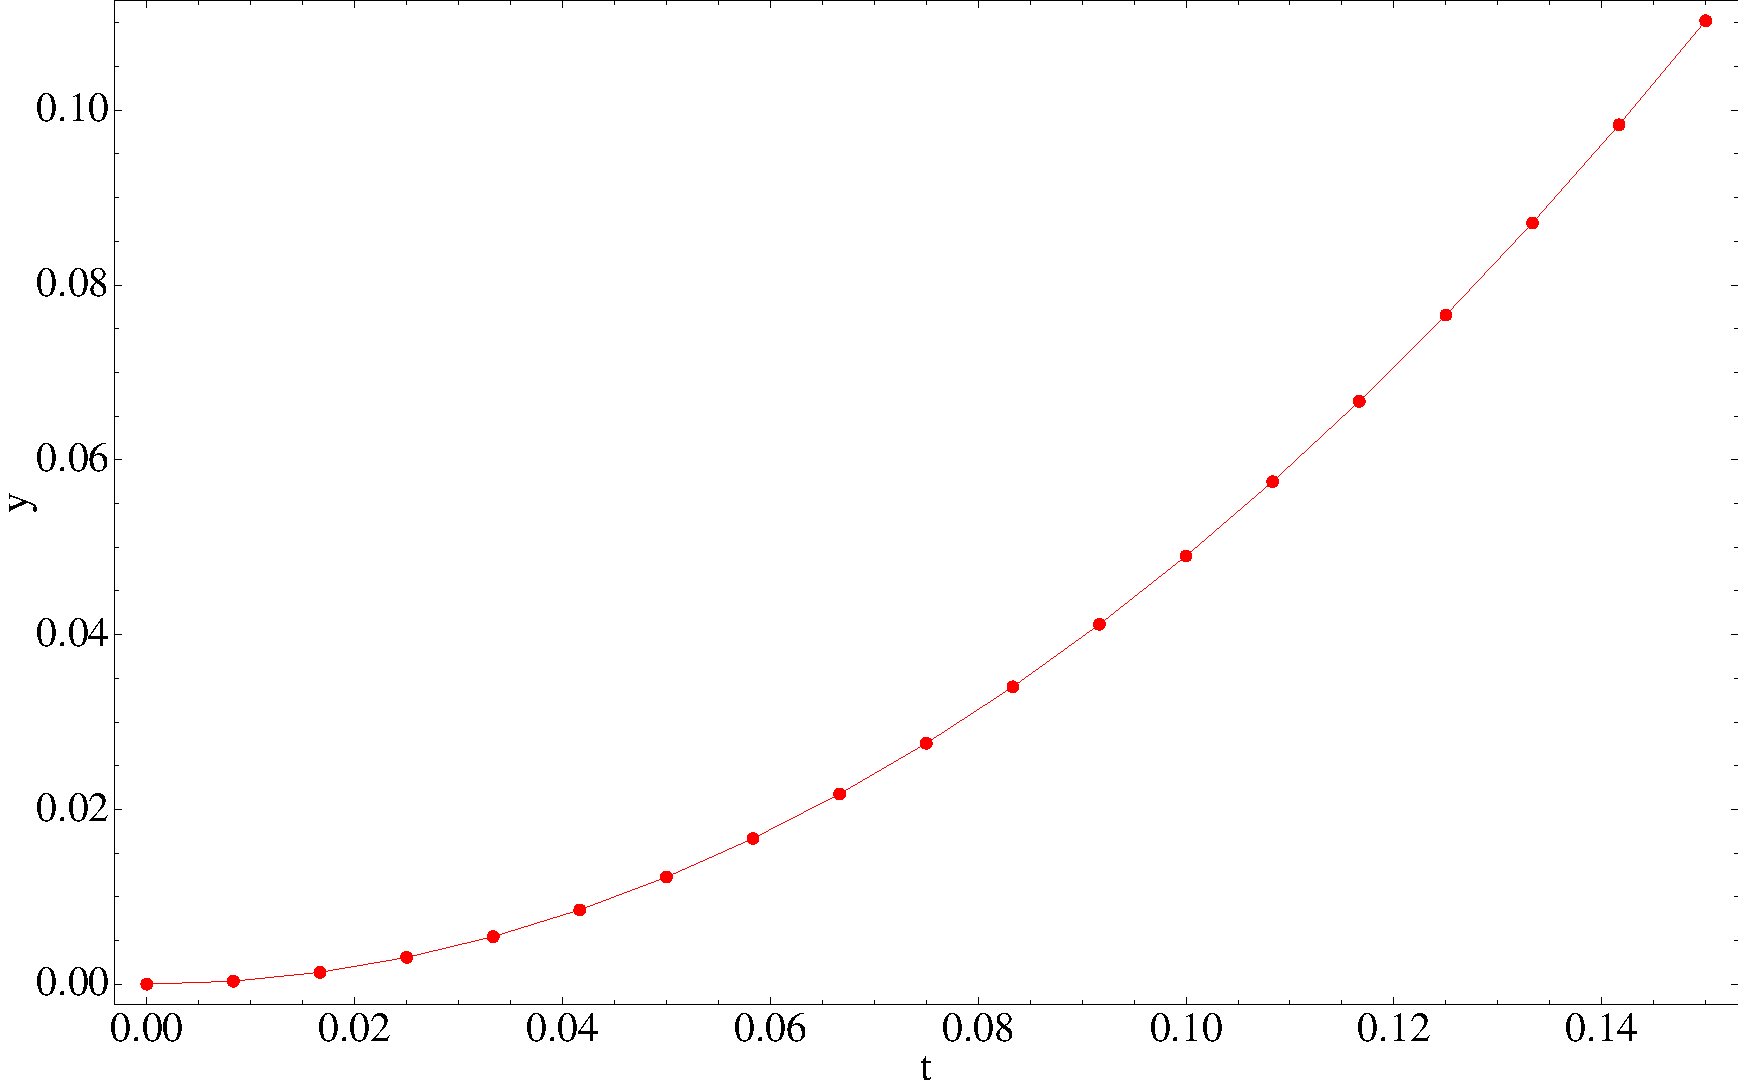
\includegraphics[width=\textwidth]{../immagini/grafici1.pdf}
 % grafici1.pdf: 861x539 pixel, 72dpi, 30.37x19.01 cm, bb=
 \caption{Grafico dei dati ottenuti}
 \label{fig:grafico_dati}
\end{figure}

Per realizzare il grafico dei dati potete utilizzare:
\begin{itemize}
 \item Matita e carta millimetrata
 \item OpenOffice.org Calc (foglio elettronico)
 \item Gnuplot \url{www.gnuplot.info}
 \item Scilab \url{www.scilab.org}
 \item Sage \url{www.sagemath.org}
\end{itemize}
\section{Calcolo numerico di velocità ed accelerazione}


Dalla teoria studiata in classe sappiamo che:
\begin{equation}
 v_x(t)=\lim _{\Delta t \to 0} \frac {\Delta x}{\Delta t}
\end{equation}
chiaramente questa formula non è applicabile ad un sistema reale dato che non è materialmente possibile effettuare misurazioni della posizione ad intervalli di tempo arbitrariamente piccoli. La velocità che andremo a calcolare sarà quindi rappresentata nel nostro grafico $(t,s)$ dalla pendenza della spezzata che congiunge due punti (misure). Il valore che otterremo dal calcolo sarà quindi una velocità media\footnote{
La formula [\ref{forward_diff}] è detta differenza in avanti, utilizzando tre punti (la così detta differenza centrale) è possibile ottenere un risultato più accurato nel calcolo della velocità }:
\begin{equation}\label{forward_diff}
\overline{v}_x(t_i)=\frac{\Delta x}{\Delta t}=\frac{x_{i+1}-x_i}{\Delta t}
\end{equation}
Una volta ottenuta la velocità media possiamo calcolare l'accelerazione media utilizzando una formula analoga alla [\ref{forward_diff}]:
\begin{equation}
 \overline{a}_x(t_i)=\frac{\Delta v}{\Delta t}=\frac{v_{i+1}-v_i}{\Delta t}
\end{equation}
Al termine dei calcoli riporteremo i risultati ottenuti in una tabella e quindi in un grafico che ci aiuterà a visualizzare la dipendenza temporale di accelerazione  e velocità:
\begin{table}[H]
\begin{center}
\begin{tabular}{llll}\toprule
$t_i$ & $x_i$& $\overline{v}_i$& $\overline{a}_i$ \\ \midrule
$0.1s$&$0.3m$&$1ms^{-1}$&$10ms^{-2}$\\
$0.2s$&$0.4m$&$2ms^{-1}$&\ldots\\
$0.3s$&$0.6m$&\dots&\ldots\\
\ldots &\ldots&\dots&\dots \\ \bottomrule
\end{tabular}\caption{Tabella con velocità ed accelerazioni calcolate dalle misurazioni effettuate in laboratorio, notate come con $n$ misure sia possibile calcolare $n-1$ velocità ed $n-2$ accelerazioni}\label{tab:extab1}
\end{center}
\end{table}



\end{document}
